\documentclass{report}
\usepackage[utf8]{inputenc}
\usepackage{graphicx}
\usepackage{caption}
\usepackage{blindtext}
\usepackage{hyperref}
\usepackage{subcaption}
\usepackage{fancyhdr} % Import fancyhdr package
\usepackage{lipsum} % Generate random filler text
\usepackage{titlesec} % Load titlesec package
\usepackage{geometry} % Access extensive page dimension controls
\usepackage{listings}
\usepackage{bookmark}
\usepackage{array}

\geometry{
  margin = 1in % Sets equal margins for all sides (modify as desired)
}

\titleformat{\chapter}[hang]
  {\normalfont\huge\bfseries}
  {\thechapter\hspace{1em}}
  {0pt}
  {\bfseries}


\pagestyle{fancy} % Enable custom headers and footers
\fancyhf{} % Reset header and footer fields
\fancyhead[RE,RO]{Nathan Vanbeselaere - Arthur Macdonald} % Top-right header field
\renewcommand{\footrulewidth}{0pt} % Remove separator line

\title{\textbf{\Huge Rapport de Projet Compilation }}
\author{Nathan Vanbeselaere - Arthur Macdonald}
\date{Avril 2024}

\begin{document}

\maketitle
\newpage

\tableofcontents
\newpage

\chapter{Réponses aux questions}

    \section{Questions sur le Lexer}

        Pour traiter les commentaires sur plusieurs lignes, on crée un nouvel état dans lequel on incrémente le buffer à chaque retour a la ligne et qui s'arrete seulement lorsqu'il rencotre les charactères "*/". 

    \section{Questions sur le Parser}
    
    \quad 1. On consid`ere la séquence suivante : If \#expr\# If \#expr\# \#stmt\# Else \#stmt\#
\quad On consid`ere pour cette question que \#expr\# et \#stmt\# sont des terminaux (i.e., onne cherchera pas à les "étendre").\\
    
    \quad (a) Donnez les deux arbres de dérivations possible de cette séquence dans la gram-
    maire décrite plus haut.

    \begin{figure}[h]
        \centering
      \begin{subfigure}{0.45\textwidth}
        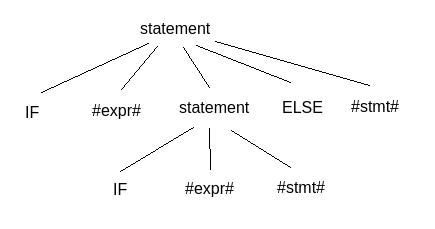
\includegraphics[width=\linewidth]{ArbreIFIFELSE1.png}
        \caption{Arbre 1}
      \end{subfigure}
      \hspace{1cm}
      \begin{subfigure}{0.45\textwidth}
        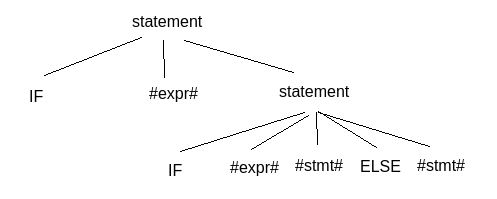
\includegraphics[width=\linewidth]{ArbreIFIFELSE2.png}
        \caption{Arbre 2}
      \end{subfigure}
    \end{figure}

    \quad (b) Donnez l'état de l'automate LR0 o`u apparaît le conflit qui montre l'existence
    de ces deux arbres.\\

    \quad L'état de l'automate LR(0) où apparaît le conflit qui montre l'existence de ces deux arbres est celui où l'analyseur doit choisir entre reduce avec un second If ou shift avec un Else.\\

    \quad (c) Quelle annotation permet d'obtenir l'arbre cohérent avec la priorité décrite dans
    ce document ?\\

    \quad  Pour obtenir un arbre cohérent avec la priorité décrite dans le document, il faut ajouter l'annotation "\%nonassoc ELSE” pour que le Else se rattache toujours au If non-terminé le plus proche puis “\%nonassoc IFELSE” avec “\%proc IFTHEN” sur la règle IF sans ELSE. Ainsi, cela nous permet d'obtenir un seul et unique arbre.\\

    \quad (d) Pouvez-vous via une annotation obtenir le comportement inverse ? Pourquoi ?\\

    \quad Non, il n'est pas possible d'obtenir le comportement inverse via une annotation car si l'on priorise la règle IF sans ELSE, on se retrouvera à un moment donné avec un ELSE libre qui ne se relie à aucune configuration de l'automate.\\

    \quad 2. Choisissez un conflit shift-reduce possible dans votre grammaire sans annotation (qui
    n'est pas celui de la question précédente), et expliquez quelles annotations de priorité
    vous avez mis pour le résoudre, et son effet sur les arbres acceptés (quels arbres sont
    privilégiés, lesquels sont ignorés). Vous illustrerez un exemple o`u ce conflit pourrait
    arriver et les deux arbres mis en jeu via une séquence de tokens.\\

    \quad Les operateurs binaires BINOP (par exemple PLUS) ont des conflits shift reduce avec les expressions.\\

    \quad Exemple avec "\#expr\# PLUS \#expr\# PLUS \#expr\#"  :\\

    \begin{figure}[h]
        \centering
      \begin{subfigure}{0.45\textwidth}
        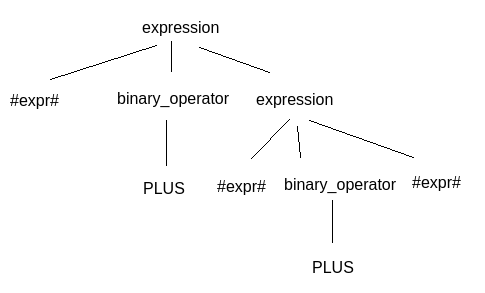
\includegraphics[width=\linewidth]{ArbrePLUSPLUS1.png}
        \caption{Arbre 1}
      \end{subfigure}
      \hspace{1cm}
      \begin{subfigure}{0.45\textwidth}
        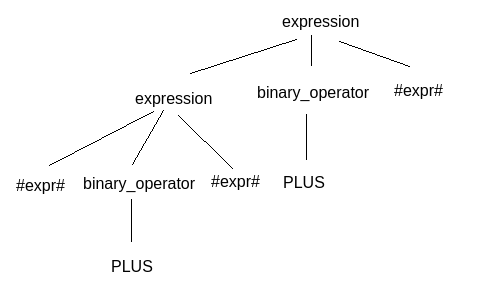
\includegraphics[width=\linewidth]{ArbrePLUSPLUS2.png}
        \caption{Arbre 2}
      \end{subfigure}
    \end{figure}
    
    Pour résoudre ce conflit, on ajoute les annotations "\%nonassoc BINOP" et "\%left PLUS" pour donner la priorité au shift ainsi seul l'Arbre 1 sera accepté.\\

    \newpage

    \section{Questions passe renommage}
    \quad 1. Pourquoi n'est-il pas gênant que dans deux blocs disjoints (pas l'un dans l'autre) un même nom soit utilisé pour des variables locales à ces blocs ?\\ 
    
    \quad Il n'est pas gênant que dans deux blocs disjoints un même nom soit utilisé pour des variables locales à ces blocs car les variables locales sont déclarées dans des environnements différents. Ainsi, les variables locales de deux blocs disjoints n'ont pas de lien entre elles et ne peuvent pas être confondues.\\

    2. Dans le programme suivant (il s'agit du programme renaming.pix, qui n'a pas d'intérêt particulier autre que pour cet exercice), indiquez comment le renommage des variables sera effectué :\\
    
    \begin{lstlisting}[language=C, basicstyle=\ttfamily]
    Program after analysis:
    Arguments <
      Int : x;
      Real : y
      >
    $<
        Set(x, (2*x));
        Real : x#1;
        Set(x#1, (2.*y));
        Int : y#1;
        Set(y#1, Floor(x#1));
        $<
            Int : x#2;
            Set(x#2, (2*y#1));
            Int : y#2;
            Set(y#2, (2*x#2));
            
        >$;
        Set(y#1, (2*y#1));
        $<
            Coord : x#2;
            Set(x#2, Coord(y#1, y#1));
            Color : y#2;
            Set(y#2, Color(x#2.X, x#2.X, x#2.X));
            Draw_pixel(Pixel(x#2, y#2));
            
        >$;
        Set(x#1, (2.2*x#1));
        
    >$
    \end{lstlisting}

    \newpage


    \section{Questions passe typage}

    \quad 1. Pourquoi a-t'on besoin de Type\_generic pour la liste vide ?\\

    \quad Type\_generic est utilisé pour la liste vide car la liste ne possède pas de type défini. On utilise donc Type\_generic comme type par défaut, qui sera modifié ensuite lorsqu'une première variable sera insérée dans le tableau. Le type du tableau deviendra donc ensuite le type de cette meme variable.\\

    2. Pourquoi doit-on réaliser des copies des environnements avant de vérifier la cohérence
        des types `a l'intérieur des blocs ?\\

    \quad Il est primordial de réaliser des copies des environnements afin d'éviter d'affecter l'environnement global de manière non voulue. En effet, lors de la vérification des types à l'intérieur d'un bloc, il est parfois nécessaire de réaliser des modifications. Or, en copiant l'environnement, vous pourrez modifier celle-ci sans pour autant modifier l'environnement global. \\

    3. Donnez un tableau similaire `a celui des opérateurs unaires qui précise le typage des
        champs (fields).\\

        \begin{tabular}{| c | c | c |}
            \hline
            AST & Type compatible & Type de sortie \\
            \hline
            Color & Type\_pixel & Type\_color \\
            \hline
            Coord & Type\_pixel & Type\_coord \\
            \hline
            X & Type\_coord & Type\_int \\
            \hline
            Y & Type\_coord & Type\_int \\
            \hline
            Red & Type\_color & Type\_int \\
            \hline
            Green & Type\_color & Type\_int \\
            \hline
            Blue & Type\_color & Type\_int \\
            \hline
        \end{tabular}\\

    4. Expliquez quelles sont les deux erreurs qu'on peut détecter lorsqu'on traite un state-
        ment For(x,start,last,step,body) lors de l'analyse de type.\\

        La première erreur est :\\
        \begin{verbatim}
            "For loop on %s instead of Int or Real"
        \end{verbatim}
        \quad Qui est détecter lorsque les types de “start” n’est ni un “Int” ni un “Real”.\\
        \newline
        \newline
        \quad La deuxième erreur est :\\
        \begin{verbatim}
            "For loop with inconsistent types %s, %s and %s"
        \end{verbatim}
        \quad Qui est détecter lorsque les types de “start”, “last” et “step” ne sont pas identiques.\\

    \newpage

    \section{Questions passe simplification de terme}

    \quad 1. Pourquoi peut-on éliminer les For dans le cas décrit ci-dessus ? \\

    Il est possible d'éliminer les boucles For, car si notre borne de départ est strictement supérieure à notre borne d'arrivée, alors aucune itération n'est possible. Par conséquent, la boucle est inutile et peut être remplacée par un bloc vide. \\

    2. Pourquoi ne simplifie t'on pas les nœuds de la forme Real\_of\_int(Floor(n,a1),a2)? \\

    On ne simplifie pas les nœuds Real\_of\_int(Floor(n,a1),a2), car ceux-ci représentent une conversion vers un nombre réel. En simplifiant ce nœud, le résultat obtenu pourrait être différent du véritable résultat. Il est donc nécessaire de garder la structure de ces nœuds, afin d'éviter des erreurs de calculs et de typage.\\

    \section{Extension}

    \newpage

\chapter{Difficultées rencontrées}

   \quad Nous n'avons pas rencontré de difficultées particulières lors de l'implémentation du lexer, du parser ou de la passe renommage.\\

    \section{Passe simplification de terme}

    \section{Extension}

\end{document}